\documentclass[a4,paper,fleqn]{article}

\usepackage{layout}

\DeclareSIUnit\year{Jahr}
\newcommand{\wye}{
    \begin{tikzpicture}
        \draw ( 90:0) -- ( 90:0.2);
        \draw (210:0) -- (210:0.2);
        \draw (330:0) -- (330:0.2);
    \end{tikzpicture}
}

\title{Notizen EEV -- SW02}
\date{\today}
\author{Daniel Winz}

\begin{document}
\maketitle
\clearpage

\section{Neutralleiterspannung}
\[ \underline{U}_{KN} =
    \frac{
        \frac{\underline{U}_{1N}}{\underline{Z}_{1}} +
        \frac{\underline{U}_{2N}}{\underline{Z}_{2}} +
        \frac{\underline{U}_{3N}}{\underline{Z}_{3}}
    }
    {
        \frac{1}{\underline{Z}_{1}} +
        \frac{1}{\underline{Z}_{2}} +
        \frac{1}{\underline{Z}_{3}} +
        \frac{1}{\underline{Z}_{N}}
    }
\]
\begin{figure}[h!]
    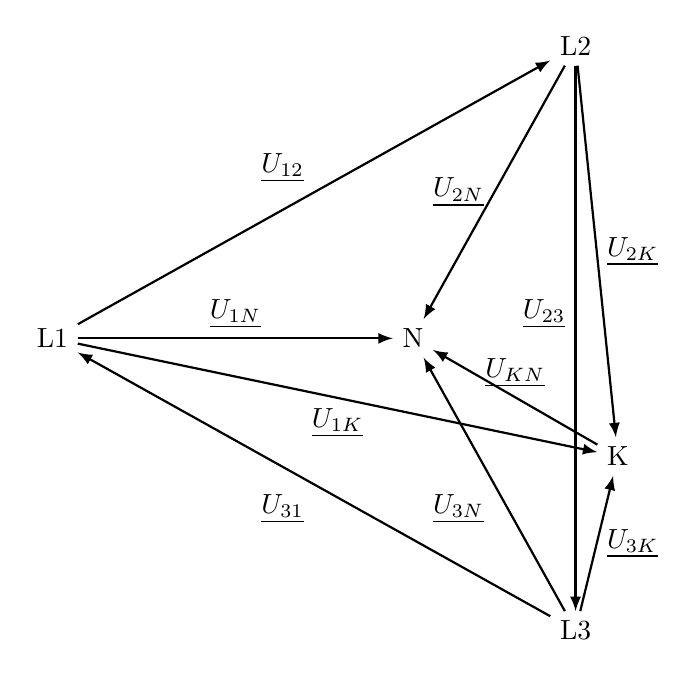
\begin{tikzpicture}
        \node(l1) at (180:4) [left]        {L1};
        \node(l2) at ( 60:4) [above right] {L2};
        \node(l3) at (300:4) [below right] {L3};
        \node(n)  at (  0:0) [right]       {N};
        \node(k)  at (330:3) [right]       {K};
        \draw[thick, -latex] (l1) -- node[above left] {$\underline{U_{12}}$} (l2);
        \draw[thick, -latex] (l2) -- node[above left] {$\underline{U_{23}}$} (l3);
        \draw[thick, -latex] (l3) -- node[below left] {$\underline{U_{31}}$} (l1);
        \draw[thick, -latex] (l1) -- node[above]      {$\underline{U_{1N}}$} (n);
        \draw[thick, -latex] (l2) -- node[left]       {$\underline{U_{2N}}$} (n);
        \draw[thick, -latex] (l3) -- node[below left] {$\underline{U_{3N}}$} (n);
        \draw[thick, -latex] (l1) -- node[below]      {$\underline{U_{1K}}$} (k);
        \draw[thick, -latex] (l2) -- node[right]      {$\underline{U_{2K}}$} (k);
        \draw[thick, -latex] (l3) -- node[right]      {$\underline{U_{3K}}$} (k);
        \draw[thick, -latex] (k)  -- node[above]      {$\underline{U_{KN}}$} (n);
    \end{tikzpicture}
\end{figure}

\section{Vorteile des Drehstroms}
\begin{itemize}
    \item 2 Spannungen verfügbar: \\
        $U_{S}$ und $\sqrt{3} \cdot U_{S} = U$ verkettet
    \item Erzeugung eines Drehfeldes (Drehfeldmaschinen)
    \item Weniger Leitermaterial im Vergleich zur einphasigen Übertragung
    \item Bei symmetrischer Belastung ist die Wirkleistung zeitlich konstant (alle 3 Phasen zusammen)
\end{itemize}

\section{Symmetrische Belastung}
Überall $\underline{Z} = Z \angle\varphi_Z$

\subsection{Sternschaltung (mit oder ohne Neutralleiter)}
\begin{itemize}
    \item Strangspannungen = Phasenspannung
        \[ U_{1K} = U_{2K} = U_{3K} = \frac{U}{\sqrt{3}} = U_S \]
    \item Strangströme = Aussenleiterströme
        \[ I_1 = I_2 = I_3 = \frac{U_S}{Z} = I \]
    \item Scheinleistung
        \[ S = 3 \cdot U_s \cdot I = 3 \cdot \frac{U}{\sqrt{3}} \cdot I = \sqrt{3} \cdot U \cdot I \]
        \[ \boxed{S = \sqrt{3} \cdot U \cdot I \qquad 
            \underline{S} = \sqrt{3} \cdot U \cdot I \angle \varphi_Z} \]
\end{itemize}

\subsection{Dreieckspannung}
\begin{itemize}
    \item Strangspannungen = verkettete Spannungen
        \[ U_{12} = U_{23} = U_{31} = U \]
    \item Strangströme
        \[ I_{12} = I_{23} = I_{31} = \frac{U}{Z} = I_{\triangle} \]
    \item Aussenleiterströme
        \[ I_1 = I_2 = I_3 = \sqrt{3} \cdot I_{\triangle} = I \]
    \item Scheinleistung
        \[ S = 3 \cdot U \cdot I_{\triangle} = 3 \cdot U \cdot \frac{I}{\sqrt{3}} = \sqrt{3} \cdot U \cdot I \]
        \[ \boxed{S = \sqrt{3} \cdot U \cdot I \qquad 
            \underline{S} = \sqrt{3} \cdot U \cdot I \angle \varphi_Z} \]
\end{itemize}

\section{Leistungsvergleich $\star$ - $\triangle$}
\begin{tabular}{ll}
    $\star$:     & $S_{\star} = \dfrac{U^2}{Z}$ \\ 
    $\triangle$: & $S_{\triangle} = 3 \cdot \dfrac{U^2}{Z}$ \\
\end{tabular}
\[ \Rightarrow S_{\triangle} = 3 \cdot S_{\star} \]
\[ \Rightarrow P_{\triangle} = 3 \cdot P_{\star} \]
\[ \Rightarrow Q_{\triangle} = 3 \cdot Q_{\star} \]

\end{document}
